% options:
% thesis=B bachelor's thesis
% thesis=M master's thesis
% czech thesis in Czech language
% english thesis in English language
% hidelinks remove colour boxes around hyperlinks

\documentclass[thesis=M,czech]{FITthesis}[2013/05/10]

\usepackage[utf8]{inputenc} % LaTeX source encoded as UTF-8

\usepackage{graphicx} %graphics files inclusion
% \usepackage{amsmath} %advanced maths
% \usepackage{amssymb} %additional math symbols

\usepackage{dirtree} %directory tree visualisation

% % list of acronyms
% \usepackage[acronym,nonumberlist,toc,numberedsection=autolabel]{glossaries}
% \iflanguage{czech}{\renewcommand*{\acronymname}{Seznam pou{\v z}it{\' y}ch zkratek}}{}
% \makeglossaries

\newcommand{\tg}{\mathop{\mathrm{tg}}} %cesky tangens
\newcommand{\cotg}{\mathop{\mathrm{cotg}}} %cesky cotangens

% % % % % % % % % % % % % % % % % % % % % % % % % % % % % % 
% ODTUD DAL VSE ZMENTE
% % % % % % % % % % % % % % % % % % % % % % % % % % % % % % 
\usepackage{listings}
\parskip = \baselineskip
\hyphenation{nej-ví-ce}
\hyphenation{dy-na-mic-ké-mu}
\hyphenation{zpra-co-vá-ní}
\hyphenation{po-li-tic-kým}
\hyphenation{na-pří-klad}


\department{Katedra softwarového inženýrství}
\title{Automatizace interakcí na sociální síti Facebook}
\authorGN{Jakub} %(křestní) jméno (jména) autora
\authorFN{Škvára} %příjmení autora
\authorWithDegrees{Bc. Jakub Škvára} %jméno autora včetně současných akademických titulů
\supervisor{Ing. Jaroslav Kuchař}
\acknowledgements{Chtěl bych poděkovat svému vedoucímu Ing. Jaroslavu Kuchařovi, za ochotu a pomoc při psaní této diplomové práce.}
\abstractCS{V~několika větách shrňte obsah a přínos této práce v~češtině. Po přečtení abstraktu by se čtenář měl mít čtenář dost informací pro rozhodnutí, zda chce Vaši práci číst.}
\abstractEN{Sem doplňte ekvivalent abstraktu Vaší práce v~angličtině.}
\placeForDeclarationOfAuthenticity{V~Praze}
\declarationOfAuthenticityOption{1} %volba Prohlášení
\keywordsCS{Nahraďte seznamem klíčových slov v češtině oddělených čárkou.}
\keywordsEN{Nahraďte seznamem klíčových slov v angličtině oddělených čárkou.}

\begin{document}

% \newacronym{CVUT}{{\v C}VUT}{{\v C}esk{\' e} vysok{\' e} u{\v c}en{\' i} technick{\' e} v Praze}
% \newacronym{FIT}{FIT}{Fakulta informa{\v c}n{\' i}ch technologi{\' i}}

%\begin{introduction}
%\end{introduction}

\chapter{{\' U}vod}
\section{Motivace}
- prinos
- zminit paper
- fb, problemy, vek …
- zamereni na facebook
- cile prace
- prinos
- cz prostredi
- fb vs tw - vice moznosti na FB, znamejsi mezi mladymi
FIT
= co je fb = soc sit apod
- vse je popisovano k datu duben 2013, muze se menit a meni,



\chapter{Analýza}

Před začátkem celého experimentu jsem prošel různé možnosti, kterými by šel experiment nejlépe realizovat. Zjišťoval jsem možnosti a omezení dostupných nástrojů a sledoval jsem výhody a nevýhody možných řešení. 

\section{Možností interakcí s facebookem}

\subsection{Rozhraní internetové stránky facebook}
Pro interakci s facebookem používá většina uživatelů webové rozhraní, které je na webové adrese \verb|www.facebook.com|. Toto rozhraní je upraveno pomocí techniky takzvaného responzivního designu\footnote{http://en.wikipedia.org/wiki/Responsive\_web\_design} pro různé typy zařízení, takže se zobrazuje jedno rozhraní stránky pro monitory osobních počítačů s velkým rozlišením a odlišný design pro chytré telefony a tablety s malými displeji a s~nízkým rozlišením. Většina uživatelů je na toto rozhraní zvyklá a to i přesto, že jej facebook často drasticky mění bez možnosti návratu ke starší verzi designu. 

Dříve se kvůli změnám rozhraní nejednou zvedla velká vlna nevole (například změna osobních profilů v roce [todo citace] 2009\footnote{http://www.zive.cz/bleskovky/facebook-tento-tyden-ceka-velka-zmena-priblizi-se-twitteru/sc-4-a-146045/default.aspx}, změna zobrazení facebookové zdi v~roce  2010\footnote{http://www.zive.cz/bleskovky/facebook-opet-v-novem-kompletni-zmena-okoli-zdi/sc-4-a-150779/default.aspx}, zavedení timeline v roce 2011\footnote{http://computerworld.cz/internet-a-komunikace/facebook-chrli-dalsi-novinky-rozsiruje-moznosti-profilu-43866} anebo přepracování zpráv v roce 2012\footnote{http://www.cnews.cz/clanky/facebook-se-chysta-prepracovat-zpravy-budou-se-vice-podobat-e-mailu}). Nyní se kvůli těmto problémům snaží facebook oznamovat předem veřejnosti výhody a nové možnosti úprav designu a zapíná nové funkce postupně s možností dočasně používat starou verzi.  

\subsection{Facebook Graph API}
Druhou možností, jak používat facebook jsou aplikace. Většinou se jedná o aplikace pro chytré telefony, tablety a další zařízení. Tyto aplikace komunikují s facebookem pomocí takzvaného \textbf{Graph API}\footnote{https://developers.facebook.com/docs/reference/apis/}. [todo citace] Jedná se o RESTové webové rozhraní.

Přihlašování ke Graph API se provádí následujícím způsobem. Každá aplikace má přiřazen svůj vlastní veřejný klíč (API Key), sloužící jako jednoznačný identifikátor (ID) aplikace a dále tajný neveřejný klíč (takzvaný APP Secret), pomocí kterého se k aplikaci příhlašuje. Každý uživatel, který chce aplikaci používat, musí danou aplikaci schválit na svém facebookovém profilu a povolit oprávnění, jaká data může aplikace číst a měnit.

Celý proces přihlašování k facebooku používá OAuth autorizaci\footnote{http://oauth.net/}\footnote{https://developers.facebook.com/docs/howtos/login/server-side-login/}, při které je uživatel aplikace přesměrován na stránky facebooku, zde se musí uživatel příhlásit a při prvním použití aplikace povolit přístup dané aplikaci k uživatelovu profilu a datům. Poté je uživatel přesměrován na naše stránky a aplikace dostane token, pomocí kterého se identifikuje při každé další komunikaci s REST rozhraním  (jak je vidět na obrázku \ref{fig:oAuthDiagram}). Podrobnější popis příhlašování se všemi detaily je popsán na stránkách facebooku v dokumentaci \newline(https://developers.facebook.com/docs/concepts/login/login-architecture/). 

\begin{figure}[h]
\begin{center}
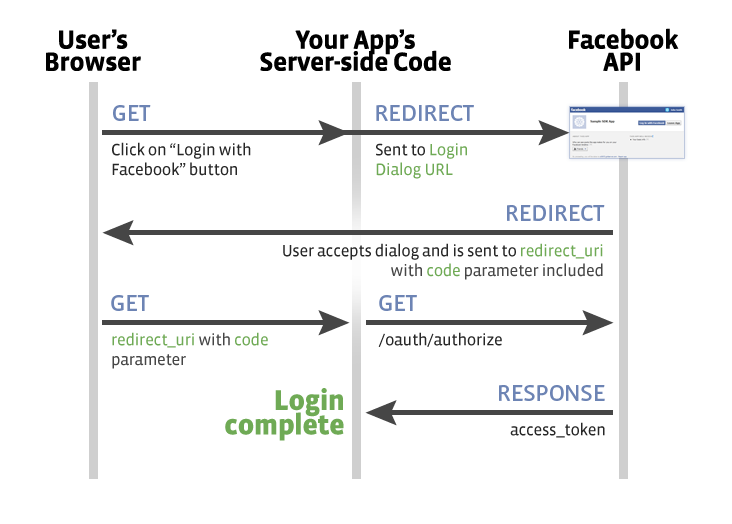
\includegraphics[width=5in]{figures/server-side-diagram.png}
\caption{Schéma přihlašování k facebooku pomocí OAuth}
(https://developers.facebook.com/docs/concepts/login/login-architecture/)
\label{fig:oAuthDiagram}
\end{center}
\end{figure}

Existují různé knihovny pro práci s facebook Graph API, liší se hlavně použitou platformou (Google Android, Apple iOS, ...) a programovacím jazkem (serverové: PHP, Java, apod., klientské: JavaScript). Některé z těchto knihoven mohou mít přihlašovací proces kvůli omezením mírně odlišný (například JavaScript), ale hlavní princip zůstává vždy stejný.

Nemusí se vždy jednat pouze o aplikace pro interakci s facebookem, velké množství aplikací (například hry a podobné aplikace) data z facebooku pouze čtou a získávájí informace o přátelích uživatele a podobně. Takovéto aplikace jsou pak zobrazeny v okně facebooku (vložení stránky pomocí tagu iframe) a mohou používat facebookové prvky (tlačítka, vyskakovací okna, apod.\footnote{https://developers.facebook.com/docs/plugins/}), takže méně zkušený uživatelé si ani nemusí neuvědomit, že používají aplikaci, která není vyvíjena facebookem. 

Facebook nepodporuje žádnou jinou možnost, jak aplikaci ovládat kromě Graph API. Kvůli častému zneužívání tohoto API byl ale facebook postupem času nucen některé funkce tohoto rozhraní omezit nebo úplně zakázat. Jedná se hlavně o možnost dát skupině nebo stránce na facebooku like anebo přidat si přátele. Tato funkce API byla ještě spolu s takzvaným likejackingem\footnote{Variace clickjacingu, pomocí HTML, CSS anebo JavaScriptu je na stránce skryto facebookové tlačítko like a je překryto jiným tlačíkem, uživatel pak po kliknutí na viditelné tlačítko nevědomky aktivuje i skryté facebookové like tlačítko http://en.wikipedia.org/wiki/Clickjacking\#Likejacking} často zneužívána k podvodnému navyšování fanoušků facebookových skupin. 

Na internetu se dnes běžně objevují nabídky na nákup fanoušků do facebookových skupin (příklady viz tabulka \ref{tab:likes-buy}). Ve většině případů se jedná o falešné nebo ukradené facebookové účty. Některé stránky jdou ale ještě dále a nabízejí na internetu možnost koupit si na facebooku falešnou přítelkyni (\verb|www.girlfriendhire.com|, \verb|namorofake.com.br| a další). Možnosti jsou různé od nákupu statusů na vaši zeď nebo s vašim ozančením až po přidání do vztahu na facebooku. Nabízí se otázka, kolik účtů, které služby nabízí, je pravých a jaká je záruka, že po převodu peněz účty nezmizí. Každopádně se jedná o zajímavý typ businessu.


\begin{table}[h]
\centering
\caption{Příklady webových stránek sloužících pro nákup Like do skupin na facebooku}\label{tab:likes-buy}
\begin{tabular}{| l | c | p{5cm} | c |}
	\hline
	\textbf{Stránka} & 
	\textbf{Cena} \\ \hline
	
	http://get-likes.com/facebook-likes-store/ &
	1000 fanoušků za 30\$ \\ \hline
	
	http://fblikesmart.com/ &
	1000 fanoušků za 50\$ \\ \hline
	
	http://officialfacebooklikes.com/ &
	1000 fanoušků za 80\$ \\ \hline
\end{tabular}
\end{table}


Facebook proto zrušil možnost dávat stránkám like skrze Graph API. S~dalším zneuživáním funkcí facebook API se může stát, že budou dále zakázány i některé další funkce. Využití facebook API je tedy poněkud omezené a s nejistou budoucností. Hlavní nedostatky facebook Graph API pro využití pro experimentální aplikaci jsou:

\begin{itemize}
  \item nemožnost dát like skupině
  \item nemožnost přidat si nové přátele
  \item omezený výpis informací o osobě oproti webovému rozhraní
  \item časem mohou být zakázány nebo omezeny některé funkce
\end{itemize}

Tyto nedostatky Graph API mi nedovolovaly jej použít pro implementaci  aplikace pro experiment. Kvůli těmto omezením jsem si tedy vybral raději možnost obsluhovat facebook pomocí webového rozhraní za použití specializovaných programů a nástrojů k tomu určených.

\section{Možnosti ovládání webového rozhraní facebooku}

\subsection{Využití HTTP protokolu}

Jako první možnost ovládání webového rozhraná facebooku se nabízelo simulovat webový prohlížeč pomocí HTTP požadavků. Toto řešení je poměrně přímočaré a webový protokol HTTP je velmi dobře zdokumenovaný a jednoduše používatelný, později jsem ale tuto možnost zavrhnul, jelikož bych musel znovu implementovat již hotové řešení, kde bych musel řešit nízkoúrovňové problémy HTTP komunikace. 

Použití HTTP protokolu by se nejvíce vyplatilo u statických webových stránek. Největším problémem tohoto přístupu je ale skutečnost, že facebook používá velké množství AJAXových\footnote{AJAX - asynchronní načítání dynamických částí webových stránek pomocí JavaScriptu (viz http://en.wikipedia.org/wiki/Ajax\_(programming))} požadavků a dynamických JavaScriptových oken, které by mohly způsobit komplikace. Ztížilo by to především získávání informací z uživatelských profilů a podobně. Například pro zobrazení příspěvků na zdi uživatele za určité období, je potřeba dosáhnout konce stránky, kde se musí kliknout na tlačítko načíst další příspěvky a tento postup se opakuje, do té doby, než dosáhneme požadovaného stáří příspěvků, stejný způsob zobrazování dalsích dat se na facebooku používá opakovaně.

Mezi další nevýhody používání HTTP komunikace patří to, že facebook pro některé části webových stránek generuje odlišný HTML kód (mění se například atributy ID u HTML značek a podobně). Nejvíce jsem se s těmito změnami setkal na hlavní stránce facebooku, kde pravděpodobně probíhá takzvané A/B uživatelské testování stránek. To znamená, že se uživatelům zobrazují různé grafické verze stránky a následně se měří rozdíly úspěšnosti konverzního poměru měřených veličin (například: počet zobrazení stránky / počet nákupů) pro jednotlivé verze
\newline(http://en.wikipedia.org/wiki/A/B\_testing).

V poslední době se začal rozšiřovat nový internetový protokol nazvaný SPDY\footnote{http://en.wikipedia.org/wiki/SPDY}, který slouží jako nadstavba nad tradičním HTTP protokolem pro rychlejší načítání stránek. Facebook tento protokol již na svých serverch používá a mohly by tak vzniknout problémy při HTTP komunikaci i když by měl být protokol SPDY teoreticky zpětně kompatibilní, nemuselo by vše být úplně bez problémů.

Kvůli těmto problémům spojeným s používáním HTTP protokolu jsem se tedy rozhodnul využít raději některé z hotových řešení a zabývat se komunikací s webovými stránkami na vyšších vrstvách. 

\subsection{Programy simulující chování webového prohlížeče}

Jako nejjednodušší z možností ovládání webového rozhraní facebookové stránky se nasklo využití programů, které simulují internetový prohlížeč. Existuje celá škála takovýchto programů. Téměř pro každý programovací jazyk existuje některý program, který dokáže zpracovávat webové stránky. Rozdíl mezi těmito programy je především v počtu a kvalitě implementovaných webových specifikací a funkcionalit.

Programy pro zobrazování webových stránek se liší především implementovaným jádrem webového prohlížeče. V následujícím seznamu je zobrazen přehled nejpoužívanějších jader pro vykreslování webových stránek.

\begin{itemize}
  \item WebKit\footnote{Webkit - http://www.webkit.org/} - Apple Safari
  \item Blink\footnote{Spolčnost Google starající se o prohlížeč Chrome v~nedávné době oznámila, že již nadále nebude používat opensource jádro WebKit, ale vytvoří vlastní fork tohoto jádra s názvem Blink -  http://en.wikipedia.org/wiki/Blink\_(layout\_engine)} - Google Chrome
  \item Gecko\footnote{Gecko - https://developer.mozilla.org/en-US/docs/Mozilla/Gecko} - Mozilla Firefox
  \item Trident\footnote{Trident - http://en.wikipedia.org/wiki/Trident\_(layout\_engine)} - Miscrosoft Internet Explorer
\end{itemize}
 
Kromě těchto nejpoužívanějších jader, které používají internetové prohlížeče, exisuje i velké množství méně známých jader a vpodstatě každý si může implementovat vlastní vykreslovací jádro pro  webové stránky.

Vykreslovací jádro ovlivňuje to, jak bude webová stránka vykreslena. Mohou se lišit i způsoby vykreslení stejné webové stránky mezi jednotlivými verzemi stejného jádra. Existují i speciálně upravená jádra pro vykreslování internetových stránek na mobilních přístrojích, které často naschvál neimplementují některé pokročilejší funkce kvůli hardwarovým nárokům mobilních zařízení a rychlosti vykreslování.

Druhým důležitým parametrem programů pro práci s webovým rozhraním internetových stánek je to, zda se webové stránky vykreslují jen v paměti počítače, nebo zda se výsledek vykresluje i na obrazovku. Existují programy, určené především pro testování webových stránek, které pouze kontrolují výskyt a pozici jednotlivých elementů, ale nedokáží stránku vykreslit, mají vše uloženo pouze v paměti. Díky tomu jsou ale i rychlejší a jsou i implementačně jednodušší. 

Různé programy pro zpracování webových stránek jsou zobrazeny v tabulce \ref{tab:web-engines}. Jedním z nejpoužívanějších programů je pravděpodobně Selenium. Používá se především pro automatické testování webových stránek a je napsán v programovacím jazyce Java. Dalším používaným programem je PhantomJs. Jak už název napovídá, je tento program napsán v jazyce JavaScript. Hojně se používá pro vykreslování dynamických částí webového rozhraní internetových stránek přímo na serveru. Je to užitečné především pokud chceme poslat webové stránky pro vyhledávací roboty, kteří mají problémy s vykonáváním JavaScriptu. Další programy uvedené v tabulce slouží především pro testování výstupu webových stránek a liší se především programovacím jazykem a rozhraním pro práci s programem.

\begin{table}[h]
\centering
\caption{Příklady programů pro zpracování webových stránek}\label{tab:web-engines}
\begin{tabular}{| l | c | p{5cm} | c |}
	\hline
	\textbf{Název} & 
	\textbf{Jádro} & 
	\textbf{Programovací jazyk/API} & 
	\textbf{Zobrazení} \\ \hline
	
	Selenium & %\footnote{http://seleniumhq.org/} & 
	Gecko & 
	Java, C\#, Ruby, Python, PHP, Perl, Haskell, REST API & 
	vykreslení \\ \hline
	
	PhantomJs & %\footnote{http://phantomjs.org/} & 
	WebKit & 
	JavaScript & 
	paměť \\ \hline
	
	WebInject & %http://www.webinject.org/
	vlastní &
	XML API &
	paměť \\ \hline
	
	HtmlUnit & %http://htmlunit.sourceforge.net/
	vlastní &
	Java &
	paměť \\ \hline
		
% http://stackoverflow.com/questions/814757/headless-internet-browser/814929#814929	
\end{tabular}
\end{table}


\section{Popis programu Selenium}

Programů zpracovávajích webové stránky je velké množství. Jeden z nejpoužívanějších nástrojů se nazývá Selenium. Původně tento program vzniknul jako nadstavba nad webovým prohlížečem Mozilla Firefox. Pomocí nainstalovaného pluginu v tomto prohlížeci jej lze ovládat pomocí programového API, které poskytuje program Selenium. 

Jedná se o Javový \verb|.jar| soubor, který se stará o spouštění a ovládání webového prohlížeče. API programu Selenium je nezávislé na programovacím jazyku a tak mohli vzniknout knihovny pro velké množství programovacích jazyků. Selenium používá webové RESTové API, takže se dají na internetu najít i neoficiální knihovny pro různé další jazyky, které nejsou podporovány přímo od výrobce tohoto programu. Dnes již existují k programu Selenium i pluginy, které umožňují místo prohlížeče Firefox používat prohlížeče Chrome, Operu, PhantomJS a další.

Hlavní výhoda programu Selenium spočívá v tom, že jsou webové stránky renderovány v reálném prohlížeči a operace, které se v prohlížeči odehrávají máme možnost vidět v reálném čase. V případě potřeby je možné převzít ruční kontrolu nad stránkou a pokračovat v interakci s webovou stránkou manuálně. 

S použitím reálného prohlížeče se pojí i výhoda optimalizace webových stránek facebooku. Stránky jsou pro reálný prohlížeč připravovány a zcela jistě jsou v něm i facebookem důkladně testovány pro správné 
zobrazování a fungování všech částí. V případě nefunkčnosti by facebook všechny nedostatky co nejdříve napravil a určitě by velmi rychle reagoval na nahlášné problémy. (Facebook o některých nahlášených problémech ví, ale kvůli tomu, že pro něj nejsou natolik důležité se s nimi nezabývá, například nefunkčnost URL pro přidání podmínek pro používaní facebookové aplikace  nahlášena v prosinci 2012 -\newline  https://developers.facebook.com/bugs/393455200735878.) 

Selenium je produkt, pod kterým se skrývá soubor několika programů, které slouží primárně k testování internetových stránek přímo v prohlížeči. Původně se jednalo jen o rozšíření (takzvaný plugin) do prohlížeče Firefox. Pomocí tohoto pluginu je možné nahrát konkrétní uživatelské chování na webové stránce (například: zadat konkrétní text do uživatelského pole, kliknout na tlačíto, otevřít novou stránku a podobně). Všechy akce se nahrávají a ukládají do souboru (s příponou \verb|.html|) a lze je jednoduše znovu opakovaně spouštět. Celý postup je totožný s používáním funkce makro pro hromadné operace v programech jako jsou Microsoft Word anebo Adobe Photoshop. Tento program se nyní nazývá Selenium~IDE\footnote{http://docs.seleniumhq.org/projects/ide/}.

Díky oblibě tohoto pluginu se postupem času utvořil kolem této technologie celý ekosystém pro automatizované testování pomocí webového prohlížeče. Do tohoto ekosystému patří následující programy:

\begin{itemize}
  \item \textbf{Selenium IDE} - plugin popsaný výše
  \item \textbf{Selenium Remote Control} - program pro ovládání prohlížeče lokálně nebo na jiných počítačích z různých programovacích jazyků
  \item \textbf{Selenium WebDriver} - program pro spouštění prohlížeče lokálně nabo na jiných počítačích
  \item \textbf{Selenium Grid} - za pomoci programu Selenium Remote Control dokáže spouštět webové prohlížeče na více serverech zároveň - hodí se především na testování stránek v odlišncýh prohlížečích a na různých operačních systémech
\end{itemize}

Více informace o jednotlivých produktech lze nalézt na oficiálnich stánkách jednotlivých programů: http://docs.seleniumhq.org/projects/. 

\subsection{Popis fungování programu Selenium WebDriver}

Pro náš experiment se nejlépe hodí program Seleinum WebDriver. Jedná se o programátorské rozhraní k ovládání celého prohlížeče z různých jazyků. Můžeme tak pomocí běžného programovacího jazyka napsat program, který spustí prohlížeč, provede v něm určené úkoly a poté prohlížeč zavře. To vše bez potřeby jakékoliv lidské interakce, takže tyto úkony mohou být opakovatelné a prováděné na různých počítačích.

Celý mechanismus funguje na jenoduchém principu. Selenium WebDriver je v podstatě jen jeden \verb|.jar| soubor\footnote{spustitelný program napsaný v programovacím jazyce Java}. Jedná se o lokální webový server, který naslouchá na určeném portu našeho počítače a vystavuje RESTové rozhraní k ovládání prohlížeče. Z našeho programu se pak můžeme připojit k webovému serveru Selenium WebDriveru a posíláme na něj požadované akce, které se mají v prohlížeči vykonat. Jelikož je webové rozhraní programu nezávislé na programovacím jazyku, existují knihovny pro mnoho jazyků a je jednoduché dopsat si i vlastní knihovnu. Program Selenium WebDriver můžeme ovládat i pomocí nástrojů pro práci s HTTP protokolem (například cURL, HTTPie, ...). Celé rozhraní je detailně popsané na stránkách projektu\footnote{https://code.google.com/p/selenium/wiki/JsonWireProtocol}.

Program Selenium WebDriver používá k ovládání prohlížeče takzvané drivery, v~tomto případě se jedná o programy, které dokáží ovládat samotný prohlížeč - otevřít jej, otevřít konkrétní URL (viz ukázka: \ref{lst:seleniumOpenUrl}) a pohybovat se po stránce (pozor, neplést s ovladači u hardware, nazývají se také drivery, ale jedná se o něco zcela jiného). Původně dokázal Selenium WebDriver ovládat pouze prohlížeč Mozilla Firefox, ale postupem času vznikly drivery i pro ostatní prohlížeče. V této době již můžeme použít Selenium WebDriver k ovládání následujících prohlížečů: Mozilla Firefox, Google Chrome, Microsoft Internet Explorer, Apple Safari, Android browser (defaultní prohlížeč na mobilních telefonech s operačním systémem Google Android), iPhone browser (defaultní prohlížeč na mobilních telefonech Apple iPhone), PhantomJS (prohlížeč implementovaný v jazyce JavaScript, běžící jen v paměti počítače), HtmlUnit (prohlížeč implementovaný v jazyce Java, běžící jen v paměti počítače). 

Mimo driverů pro webové prohlížeče existují pro program Selenium WebDriver i dva speciální drivery: EventFiringWebDriver (slouží k odchytávání JavaScriptových událostí, které v prohlížeči vzniknou, můžeme na ně pak v našem programu reagovat) a RemoteWebDriver (slouží ke vzdálenému ovládání prohlížečů na jiných počítačích). S těmito drivery máme možnost ovládat všechy hlavní internetové prohlížeče a to jak desktopové, tak i mobilní.

\begin{lstlisting}[caption={Příklad otevření url v seleniu pomocí CURL},label=lst:seleniumOpenUrl,belowcaptionskip=0.4cm]
# Pomoci tohoto prikazu vytvorime novou session 
# (otevreme prohlizec firefox)
curl -X POST http://localhost:4444/wd/hub/session \
-d "{desiredCapabilities: {browserName: 'firefox'}}"

# Z predchoziho prikazu jsme ziskali sessionId
# sessionId pouzijeme v prikazu pro otevreni stranky
# :sessionId je potreba nahradit vysledkem predchoziho
# dotazu
curl -X POST \
http://localhost:4444/wd/hub/session/:sessionId/url \
-d "{url: 'http://www.facebook.com'}" 
\end{lstlisting}

Vývojáři prohlížeče Opera vydali 12. února 2013 
článek\footnote{http://my.opera.com/ODIN/blog/300-million-users-and-move-to-webkit} o tom, že budou pro svůj prohlížeč do budoucna používat jádro WebKit, které používají prohlížeče Google Chrome a Apple Safari. Pár měsíců po tomto oznámení vydali vývojáři prohlížeče Google Chrome 3. dubna 2013 na svém webu článek\footnote{http://my.opera.com/ODIN/blog/300-million-users-and-move-to-webkit} o tom, že vytvoří vlastní vykreslovací jádro Blink\footnote{http://www.chromium.org/blink}. Bude se jednat o fork doposud používaného opensource jádra WebKit. Do budoucna bude určitě zajímavé sledovat, jak se celá situace nakonec vyvine, nicméně funkčnost programu Selenium WebDriver by to nemělo omezit.

\section{Výhody a nevýhody použití programu Selenium WebDriver}

Selenium WebDriver je program sloužící k ovládání internetového prohlížeče pomocí velkého množství programovacích jazyků. Největší výhodou používání programu Selenium WebDriver k zpracování webových stránek je, že se stará o všechnu práci spojenou s komunikací skrze HTTP protokol, vykreslováním i ovládáním webových stránek a zpracováním všech dynamických skriptů ve stránce. 

Selenium WebDriver nám umožňuje přistupovat k výsledným vyrenderovaným elementům prohlížeče a to jak textově, tak i k HTML zdrojům jednotlivých elementů na stránce. Problém nastává při následném zpracování, protože data ze stránky nejsou vždy jednotná jako v případě použití Graph API. Musíme tedy získaná data následně zpracovávat a upravovat.

Máme tedy k dispozici naprosto stejná data, jako uživatel internetového prohlížeče. Nemusíme se zabývat nízkoúrovňovými záležitostmi spojenými s fungováním internetu. Dále můžeme použít různé vykreslovací programy a webové prohlížeče a to včetně programů určených pro mobilní zařízení. Tento nástroj se nejvíce používá k automatickému testování webových stránek v různých prohlížečích a v této oblasti je velmi rozšířen. Můžeme k němu tedy nalézt velké množství návodů, knihoven, doplňků a rad na internetu. 

\textbf{Výhody využití programu Selenium WebDriver}

\begin{itemize}
  \item hojně používaný program
  \item možnost změny vykreslovacího programu
  \item velké množství vykreslovacích programů k použití
  \item možnost ručního ovládání browseru
  \item velké množství návodů, zdrojů a rad na internetu
  \item RESTové rozhraní pro ovládání browseru
  \item velké množství programátorských knihoven pro práci s tímto programem
  \item možnost přistupovat přímo k HTML zdrojům jednotlivých elementů na stránce
\end{itemize}

\textbf{Nevýhody využití programu Selenium WebDriver}

\begin{itemize}
  \item neexistuje oficiální knihovna pro jazyk PHP 
  od tvůrců programu Selenium
  \item nutnost spouštět celý browser - paměťově i časově náročnější
  oproti použití samostatné knihovny
  \item nutnost dále zpracovávat získaná data z textu nebo z HTML zdrojů elementů stránky
\end{itemize}

\section{Volba programovacího jazyka a databáze}

\subsection{Volba programovacího jazyka}

Pro implementaci celé aplikace jsem si vybral programovací jazyk PHP \footnote{Open source programovací jazyk: http://www.php.net/}. Jedná se o dynamicky typovaný programovací jazyk, který se používá především k vytváření webových stránek a internetových aplikací. Tento jazyk jsem si vybral především proto, že s ním mám osobně největší zkušenosti a přijde mi na menší aplikace ideální. 

Díky dynamickému typování lze v tomto jazyce vytvořit aplikace velmi rychle. Protože aplikace neobsahuje složitý model a hlavní funkcionalitou je převážně volání RESTových služeb a ukládání a vybírání dat z databáze, přišel mi tento jazyk jako nejlepší možnost pro implementaci programu tohoto typu.

Celá aplikace facebooku je napsána v jazyce PHP (i když používají speciální kompilátor pro tento jazyk - HipHop for PHP\footnote{HipHop for PHP - http://en.wikipedia.org/wiki/HipHop\_for\_PHP}). Mimo jiné programy facebook uvolnil k volnému používání na internetu knihovnu v PHP pro používání programu Selenium WebDriver\footnote{https://github.com/facebook/php-webdriver}. Tuto knihovnu v aplikaci také používám pro komunikaci se Selenium WebDriverem.

Při rozhodování, který programovací jazyk pro aplikaci zvolím, jsem uvažoval i o jakzyku Java, který je na rozdíl od PHP staticky typovaný. Jeho hlavní výhodou oproti jazyku PHP pro tento projekt byla knihovna přímo od tvůrců programu Selenium. Naopak nevýhodou byla nutnost výsledný program před spuštěním vždy překompilovat a tedy i pomalejší vývoj celé aplikace. Výhody jazyka Java jsou vidět až u větších a rozsáhlejších aplikací a pro takto malou aplikaci by se tyto výhody vykoupené pomalejším vývojem pravděpodobně nevyplatily. 

Mezi další nevýhody jazyka Java patří to, že pokud chceme nasadit aplikaci, je složitější sehnat hosting a je složitější nastavit celou aplikaci. Aplikaci v jazyce PHP je možné nasadit i na sdílený hosting s dalšími aplikacemi a konfigurace je jen minimální. Selenium WebDriver může běžet i na jiném serveru, protože veškerá komunikace porohíhá pomocí HTTP protokolu.

\subsection{Volba databáze}

Jako databázi pro ukládání dat jsem pro začátek zvolil MySQL. Jedná se o open source relační databázi, kterou aktuálně vlastní společnost Oracle (viz http://www.mysql.com/). Tato databáze je nejčastěji používána ve spojení právě s programovacím jazykem PHP. Do této databáze jsou ukládány informace o založených účtech, se kterými pracuje stahovací program. [V této databázi jsou také uloženy různé skupiny uživatelských účtů (například muži, ženy, apod).] 

Původně jsem chtěl pro ukládání stažených dat použít také MySQL databázi, ale rozhodl jsem se jinak. Pro ukládání dat stažených z uživatelských profilů se používá NoSQL (nerelační) databáze MongoDB. MongoDB je dnes jedna z nejrozšířenějších nerelačních databází. Jedná se o open source dokumentově orientovanou NoSQL databázi o kterou se stará společnost 10gen (http://www.mongodb.org/). Jedna z největších předností této databáze je, že do ní lze ukládat jakákoliv nestrukturovaná data ve~formátu JSON (JavaScript Object Notation - http://www.json.org/) a lze pak s těmito daty nadále manipulovat a provádět nad nimi agregační dotazy. 

Databáze MongoDB byla vybrána hlavně kvůli tomu, že umí pracovat s jaýmikoliv nestrukturovanými daty, to znamená, že cokoliv, co získáme z~facebooku můžeme rovnou uložit. Takovéto chování se hodí především k ukládání příspěvků ze~zdi facebookových uživatelů a informací z profilových stránek osob. Nemusíme se starat o to, že někteří uživatelé mají omezenou viditelnost počtu přátel nebo počtu skupin.

Facebook v roce 2010 vyvinul vlastní NoSQL databázi nazvanou Cassandra (http://en.wikipedia.org/wiki/Apache\_Cassandra), která slouží k vyhledávání nad velkým objemem dat. Facebook tuto databázi později nahradil další NoSQL databází nazvanou HBase (http://hbase.apache.org/). Tyto databáze jsou ale určeny především k vyhledávání a jejich výhoda se ukáže až při ukládání mnohem většího množství dat, než bylo pro daný experiment potřeba.





\chapter{Implementace}

\section{Rozdělení aplikace}

Aplikace sloužící pro otestování celého experimentu má dvě základní funkce. První z nich je sbírání dat o uživatelích facebooku z jejich profilů a inforamcí na jejich účtech. Druhou funkcí je ovládní fiktivních účtů, to znamená, nahrávání dat na facebook a interakce s dalšími uživateli. Data uživatelů z facebooku slouží k~analýze a k~dalšímu porovnání.

\section{Stahování informací z facebookových profilů}

Důležitou součástí aplikace je získávání informací o~uživatelích z~jejich facebookových profilů. Jak již bylo zmíněno v předchozí kapitole, vybral jsem pro stahování program Seleinum WebDriver, který je spouštěn pomocí jazyka PHP. Sesbíraná data jsou ukládána do databáze MongoDB nad kterou lze jednoduše vykonávat dotazy pro získání jakýchkoliv statistických dat.

O veškeré zpracování stránek facebooku se stará program Selenium WebDriver, pomocí kterého se načte konkrétní stránka (například zeď anebo přátelé určitého uživatele), z této stránky se poté přečtou jednotlivé fragmenty (například příspěvek na zdi anebo jméno přítele na facebooku) a tato data jsou pak pomocí PHP zpracována, upravena a uložena do databáze MongoDB. 

Facebook je celosvětová sociální síť a je tedy přeložen do velkého množství jazků (včetně pirátské angličtiny a angličtiny s písmenky vzhůru nohy). Facebook je celý primárně v anglickém jazyce a do ostatních jazyků je celá aplikace přeložena. Překlad do všech jazyků probíhá pomocí speciální facebookové aplikace (\verb|https://www.facebook.com/?app=1&sk=translations|), kam mohou své překlady zasílat všichni uživatelé facebooku. (Dříve bylo docela dlouhou dobu v českém překladu špatně přeloženo slovo neděle jako slunce - anglicky Sun = slunce a zkratka neděle.) Jazyk procházených stránek pomocí programu Selenium WebDriver byl tedy vždy nastaven na anglický jazyk, abz nedocházelo k problémům s překlady. 

Pro každý náš facebookový účet uložený v aplikaci je spuštěna následující sekvence operací:

\begin{itemize}
  \item stažení příspěvků na vlastní zdi
  \item stažení všech přátel, kteří si náš účet přidali
  \item stažení posledních příspěvků každého uživatele, kterého má účet v přátelích
\end{itemize}

\subsection{Zpracování stahovaných informací}

Všechny statusy (příspěvky na zdi uživatele), které jsou stahovány ze zdi jsou pročištěny od nedůležitých dat a upravovány do stejné podoby. Data, která jsou získávána z facebooku, jsou někdy zobrazena rozdílně. Například zobrazení like u statusů. Pro analýzu statusů potřebujeme ukládat pouze počet like, které status obdržel. Facebook bohužel ale někdy místo počtu liků zobrazuje i jména lidí, kteří like udělili. Stává se tak v případě, že like udělil, někdo z lidí, které má účet v přátelích anebo pokud je u statusu pouze jeden like.

Pro účely experimentu se ukládá ke statusu pouze počet like, který je pro nás nejdůležitější. V programu se o získání počtu like stará funkce, která sečte počet jmen a počet like u statusů a vrátí výsledný součet celkových like. 

Podobná situace nastává u komentářů u facebookových statusů. Pokud status obsahuje dva až čtyři nebo méně komentářů, tak se komentáře zobrazí i s textem. (Počet plně zobrazených komentářů se různí a není dán pevně pro každý status.) Pokud status obsahuje  více komentářů, tak se zobrazí text pouze dvou (až čtyř) posledních příspěvků v komentářích u statusu a všechny předchozí komentáře se zobrazí až po kliknutí na odkaz pro zobrazení starších komentářů. Naštěstí facebook v textu tohoto odkazu zobrazuje počet předchozích komentářů. Takže pro získání počtu komentářů nemusíme odkaz rozklikávat. 

Text dlouhých komentářů se navíc na facebooku zkracuje, pokud je příliš dlouhý. Většinou se zobrazí pouze prvních pět řádků komentáře. Pro zobrazení celého textu je potřeba rozkliknout odkaz na konci zkráceného textu a zobrazí se pokračování textu komentáře. 

Pro komentáře u skupin na facebooku se používá jiný typ zobrazení než u statusů a osobních profilů. U statusů lidí na facebooku se zobrazují komentáře chronologicky podle data vložení, jen v jedné úrovni bez zanoření a pokud chce někdo reagovat na předchozí komentář, musí označit autora předchozího komentáře pomocí znaku @ a jména jeho profilu na facebooku. U facebookových skupin se komentáře zobrazují ve dvou úrovních s jedním zanořením, to znamená, že pokud chce někdo reagovat na určitý komentář, tak se nový příspěvek odsadí, ale pouze u první reakce a je vidět jistá hierarchie. Nadále se komentáře u příspěvků skupin neřadí podle data přidání, ale podle oblíbenosti a relevance (tento algoritmus není veřejný, ale většinou rozhoduje počet like u komentářů). Stejný způsob komentářů facebook zobrazuje i u svého doplňku Facebook Comments\footnote{https://developers.facebook.com/docs/reference/plugins/comments/}, který nabízí pro ostatní webové stránky na vložení jako plugin. 

\subsection{Problémy se stahovaným časem}

Další problém při stahování dat z facebooku nastal při získávání času statusů a komentářů. Pro uživatele zobrazuje facebook na svých stránkách v různých formátech. První možností je relativní časový úsek od vložení, například: about a minute ago (přibližně před minutou), X minutes ago (před X minutami), X hours ago (před X hodinami) a podobně. Takovéto údaje se zobrazují u komentářů vložených před méně než 24 hodinami. 

Dalším zobrazovaným časovým údajem bývá: yesterday (včera), Monday (pondělí) a podobně. Jedná se o statusy a komentáře vložené před více než 24 hodinami a méně než týdnem. Poslední možností zobrazení časového údaje je přesné datum, které se zobrazuje ve formátu: 15 April (15 duben). Navíc se liší zobrazený čas u statusů a komentářů pod nimi. U starších komentářů se zobrazuje i čas vložení, například: 2 February at 16:54 (2 únor v 16.45), kdežto u statusů se zobrazuje čas jen v ojedinělých případech.

Nevýhoda takovéhoto zobrazení časových údajů je, že nejsou vůbec přesné a časový rozptyl je až 24 hodin. Zkoumal jsem proto zdrojový kód stránky, zda jsou ve stránce dostupné i další údaje týkající se času vložení statusu a komentářů. Zjistil jsem, že element obsahující čas vložení má atribut \verb|title| s textovou časovou reprezentací a atribut \verb|data-utime| s takzvaným unixovým časem (počet sekund od 1. ledna 1970), příklad elementu je vidět ve výpisu \ref{lst:timeElement}. 

\begin{lstlisting}[caption={Příklad elementu obsahující čas},label=lst:timeElement,belowcaptionskip=0.4cm]
<abbr 
  title="Tuesday, 23 April 2013 at 22:47"
  data-utime="1366750038" 
  class="timestamp livetimestamp">
    10 minutes ago
</abbr>
\end{lstlisting}

Stejné elementy používá facebook pro zborazení času u statusů a komentrářů. Zkoumal jsem vztah mezi těmito dvěma časovými údaji uvedenými u elementu. Zjistil jsem, že tyto dva časové údaje nejsou stejné. Stáhnul jsem tedy z facebooku 70 elementů s časovými údaji, z toho bylo 30 komentářů a 40 statusů. Zjistil jsem, že u 28 elementů byly údaje v rámci elementu stejné, u jednoho elementu se čas lišil o 1 hodinu, u 34 elementů byly časové údaje rozdílné o 8 hodin a u 7 elementů se čas lišil o 9 hodin. Přehledně jsou všechna data shrnuta v grafu \ref{fig:timeDifference}.

\begin{figure}[h]
\begin{center}
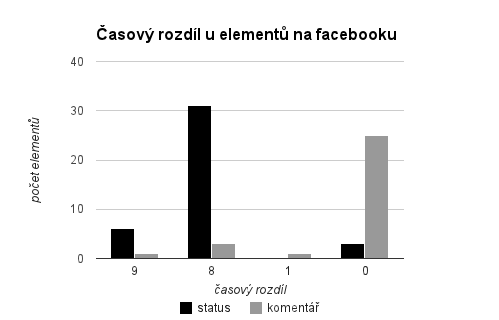
\includegraphics[width=5in]{figures/time-difference.png}
\caption{Časový rozdíl u atributů title a data-utime u elementů zobrazujících čas na facebooku}
\label{fig:timeDifference}
\end{center}
\end{figure}

U některých elementů se dokonce lišil čas o rozdílný počet hodin u statusu a odpovídajících komentářů pod ním. Tento problém bude pravděpodobně způsoben různými časovými zónami. Facebook má několik datových center po  po celém světě. Časový rozdíl 8 hodin odpovídá časovému posunu mezi západem USA a Greenwichským časem (základní časové pásmo). Rozdíl mezi Českou republikou a Greenwichským časem je pak 1 hodina. Kombinací těchto časových pousunů pravděpodobně dojde k takovýmto rozdílům, které způsobují nekonzistence mezi časy uvedenými u stejného elementu. 

Všchna data byla získána ze tří rozdílných uživatelských zdí na facebooku. Největším překvapením pro mne bylo to, že se různé rozdíly v časových údajích vyskytovaly na stejných zdech a dokonce se lišily i časové údaje u statusu a pod ním přidaných komentářích.  Je možné, že facebook vybíral statusy z jiných datových center než komentáře a tím vzniknuly takovéto nekonzistence.

Nakonec jsem po tomto zjištění otestoval, který ze dvou stahovaných časových údajů odpovídá realitě. Test byl naštěstí poměrně jednoduchý. Vše jsem vyzkoušel vložením statusu a komentáře na facebook a poté jsem kontroloval, jak se obě data liší oproti realitě. 

Z tohoto testu jsem zjistil, že realitě odpovídá údaj vložený v atributu \verb|title|, tedy textová reprezentace data vložení. Pro data ukládáná do naší databáze jsem tedy používal tuto variantu pro parsování času.

Hlavní nevýhodou použití atributu \verb|title| pro parsování data je, že datum je uloženo ve formátu: Tuesday, 23 April 2013 at 22:47. Nemáme tedy k dispozci údaj, ve které sekundě byl příspěvek vložen, ale pro náš experiment není tento údaj tolik důležitý. Pokud bychom potřebovali doplnit ve které sekundě byl status nebo komentář vložen, mohli bychom tento údaj získat z druhého atributu elementu (\verb|data-utime|). 

\subsection{Změna webového rozhraní facebooku}

Největším problémem při použití programu selenium WebDriver a vlastně jakéhokoliv programu pracujícím s webovým rozhraním facebooku je fakt, že toto rozhraní se občas mění. Někdy se jedná o změny drobné, které běžní uživatelé této sítě ani nezpozorují. Jednou za čas na facebooku ale dojde k razantnější změně webového rozhraní.

Během března 2013 facebook oznámil novou verzi profilové stránky (timeline) [todo citace http://newsroom.fb.com/News/584/Improvements-to-Timeline]. Jadnalo se o jednu z větších úprav webového rozhraní facebooku. Tato nová funkčnost byla navíc spouštěna postupně, takže někteří facebookoví uživatelé mají starou verzi timeline a některé účty již používají verzi novou. Vše funguje tak, že pokud je na vašem profilu zapnutá nová verze timeline, tak vidíte novou verzi na profilových stránkách všech vašich přátel a svojí profilové stránce. Ke staré verzi timeline se již po zapnutí facebookuem nejde nikdy vrátit. Nejde ani ovlivnit, kdy bude nová verze zapnuta právě pro váš profil.

Pro čtení dat z facebooku pomocí programu Selenium WebDriver se použíá XPath (XML Path Language). Což je jazyk pro vybírání elementů z XML a HTML dokumentů. Vše funguje tak, že se vybírají konkrétní elementy anebo se vybere konkrétní element procházejí se jeho podelementy. Konkrétní elementy se vybírají podle atributů u jednotlivých elementů.

Obával jsem se, že při změně vizuálního vzhledu timeline na facebooku budu muset předělávat velkou část stahování tak, aby aplikace mohla pracovat s novým HTML zdrohovým kódem. Naštěstí se ale HTML elementy na stránce měnily pouze minimálně. Takže stačilo upravit některé XPath dotazy a zbytek aplikace byl zcela funkční.

Změna timeline, ale měla jiný dopad. Na staré timeline se zobrazoval počet přátel, které má uživatel přidané na facebooku (pokud to neměl uživatel zakázané v nastavení). Se změnou na novou vizuální verzi timeline, ale tato položka zmizela a údaj o celkovém počtu přátel je dostupný až po přijetí přátelství od dotyčného člověka. V této chvíli tedy neexistuje žádný způsob, jak zjistit celkový počet přátel na facebooku u cizích profilů. 

\subsection{Stahovaná dat z facebooku}

Pro účely experimentu byla u statusů ukládána následující data získaná z facebooku za použití programu Selenium WebDriver:

\begin{itemize}
  \item myWall - zda byl status stažen ze zdi našeho fiktivního účtu nebo ze zdi někoho z přátel fiktivního účtu
  \item user - jméno uživatele, který status přidal
  \item fromUser - z kterého účtu byl status stažen  
  \item status - text statusu
  \item commentsCount - počet komentářů
  \item likesCount - počet like
  \item timestamp - čas vložení statusu
\end{itemize}

Dále byli ukládáni do databáze všichni přátelé. Struktura těchto dat měla byla následující:

\begin{itemize}
  \item name - Uživatelské jméno na profilu
  \item url - Url adresa profilu
  \item friendsCount - počet všech přátel stahovaného účtu, pokud to bylo možné z profilu zjistit
  \item mutual - počet společných přátel stahovaného účtu, pokud to bylo možné z profilu zjistit
  \item fromUser - kterého uživatele je stahovaný účet přítelem
  \item downloaded - čas stažení informace
\end{itemize}

[todo stahovane 3 tabulka]


\section{Nahrávání dat na facebookové profily}

Druhá část aplikace pro experiment byla určena pro nahrávání dat na fiktivní facebookvé profily. Hlavním cílem pro přidávání dat na fiktivíní profily byla simulace chování reálných uživatelů a zvýšení věrohodnosti účtů. Na facebooku je velké množství možností k interakci s ostatními uživateli. Nejdůležitějším prvkem na facebooku je zeď se statusy přátel. Statusy je možné komentovat, likovat a sdílet (poslat na svou zeď pro zviditelnění svým přátelům). 

Kromě statusů lze na facebooku komunikovat pomocí zpráv. Systém je podobný jako u e-mailových zpráv s tím rozdílem, že pomocí zpráv lze komunikovat pouze  v rámci facebooku. Dalším komunikačním kanálem je realtimový chat. Facebookový chat je propojen se zprávami, takže veškeré zprávy, které jsou poslány přes chat, jsou viditelné i ve zprávách. Výhoda chatu oproti zprávám je, že  můžeme vidět, kteří uživatelé jsou právě online a zda si zaslanou zprávu přečetli.

Hlavím cílem interakce na facebooku byla věrohodnost pro ostatní facebookové uživatele. Důležité tedy bylo zautomatizovat přidávání přátel na facebooku. Ze začátku jsem po zaregistrování nového profilu plánoval přidávat pokaždé sedm přátel. Facebook ale při přidávání většího množství přátel (většinou okolo pěti, ale někdy i méně) zobrazil potvrzovací okno \ref{fig:confirmFriendship}. Ustálil jsem tedy po tomto zjištění počet přidávaných přátel na pět za jedno přihlášení. [todo ...]

\begin{figure}[h]
\begin{center}
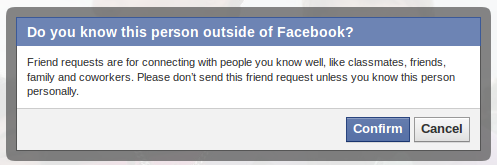
\includegraphics[width=5in]{figures/confirm-friendship.png}
\caption{Potvrzení přidání osoby do přátel na facebooku}
\label{fig:confirmFriendship}
\end{center}
\end{figure}
= ziskavani prvnich pratel

= neznami mezi sebou


Další možností, jak na sebe na facebooku upozornit určitou osobu je možnost někoho šťouchnout (poke). Funkčnost tlačítka šťouchnout je jednoduchá. Pokud vás někdo šťouchne, přijde vám upozornění a můžete šťouchnutí opětovat. Šťouchnutí je znázorněno ikonou lidské ruky s napřaženým ukazováčkem.

Pro experiment jsem sdílení omezil na přidávání statusů na svou zeď. Jedná se totiž o hlavní možnost, jak dát na facebooku o sobě vědět. Frekvence přidávání statusů byla nastavena na jeden status za přihlášení. 

Obsah vkládaných statusů byl obecný a neutrální. Jednalo se většinou o citáty a výroky známých i neznámých osobností na internetu, vtipy a neutrální a spontánní komentáře aktuálního dění (například o počasí). Jako zdroj pro statusy citátů sloužila webová stránka: \verb|citaty.net| a jako zdroj vtipných statusů sloužily stránky: \verb|www.vtipy.net|, \verb|vysmatej.cz| a \verb|vtipy.peoplelovepeople.com|. Snažil jsem se vyhýbat rasistickým a politickým vtipům, abych nepobouřil některého z přidaných přátel na facebooku. Spontánní texty statusů jsem vymýšlel sám nebo jsem se inspiroval statusy na zdi ostatních fiktivních účtů.

Ostatní typy možnosti komunikace na facebooku nebyly automaticky zpracovávány. Po přihlášení k účtu, stažení informací a spuštění automatizovaných akcí jsem vždy ručně kontroloval co se na facebookovém účtu děje. Ve většině případů se u účtu zobrazovaly notifikace o potvrzení žádostí o přátelství a několik zpráv o tom, zda náš fiktivní účet zná osobu, které byla odeslána žádost o přátelství a občas i šťouchnutí.

Facebookvé zprávy nebyly automaticky zpracovávány. Zpracovávání by totiž nepřinášelo přidanou hodnotu k našemu experimentu a zpracovávání textu by bylo složité, jak už bylo zmíněno dříve. Na žádné zprávy jsem nikdy neodpovídal. Teoreticky by bylo možné připravit univerzální odpověď na otázku, zda se dané facebookové účty znají. Například vymyšlení univerzálního místa, kde se mohly dané osoby setkat - škola, práce, apod., anebo přiznání, že se účty neznají). Pak by ale zcela určitě pokračovalo další dotazování pomocí facebookových zpráv, odkud se dané účty znají anebo proč byla odeslána žádost o přátelství na facebooku. Nejen, že by takovéto zpracovávání zabralo mnoho času a nebylo by možné plně automatizovat, ale někdy by mohlo takovéto chování být i kontraproduktivní.

= spousteno lokalne


- architektura

Chovani uzivatelu + Metriky




\chapter{Průběh experimentu}

-stahovani friend - friend dat
\section{První generace facebookových účtů}

Před samotným startem celého experimentu jsem potřeboval otestovat, jak přibližně bude vše fungovat a jak se budou účty přibližně chovat. Založil jsem proto na facebooku pět testovacích účtů, které jsem nazval \textbf{první generace}. Pomocí těchto účtů jsem zjišťoval omezení i zádrhele celého experimentu a jak by vše mělo fungovat. Pomocí těchto účtů jsem vyvíjel aplikaci pro automatické stahování a nahrávání dat na facebook (více podrobně bude celý mechanismus popsán později).

Pomocí první generace jsem ověřil, že facebook nekontroluje, pokud se z jedné IP adresy přihlašuje více účtů. Je to i logické, jelikož v institucích jako jsou školy, knihovny a podobně se může k facebooku přihlašovat více účtů, které jsou k internetu připojeny skrze jednu

\section{Příprava experimentu}

\subsection{Zakládání e-mailových adres}

Před samotným experimentem bylo potřeba založit facebookové účty pomocí kterých se bude experiment realizovat.
Zakládání falešných účtů bylo poměrně složité, jelikož jsem chtěl původně spustit celý experiment v jeden den. 
Facebook při vytváření nového účtu kontroluje vždy 
IP~adresu\footnote{IP adresa - číselná adresa počítače, pomocí které se připojuje k internetu} počítače a nedovolí ze stejné IP adresy založit více než jeden účet denně. 
Pokud se někdo pokusí založit více než jeden účet, zobrazí se na facebooku obrazovka s nutností opsat kontrolní 
CAPTCHA\footnote{CAPTCHA - jedná se o ochranu internetových stránek proti robotům, nejčastěji je realizovaná nutností opisání textu z deformovaného obrázku} obrázek a po úspěšném opsání facebook zobrazí stránku (viz obrázek \ref{fig:fbTelephoneNubmer}) s polem pro zadání telefonního čísla, na které má být zaslán aktivační kód.
Nepokoušel jsem se pak už dále dostat přes tento krok, jelikož telefonní čísla se složitě shání a jedná se o osobní údaj, který jsem nechtěl facebooku sdělovat.

\begin{figure}[h]
\begin{center}
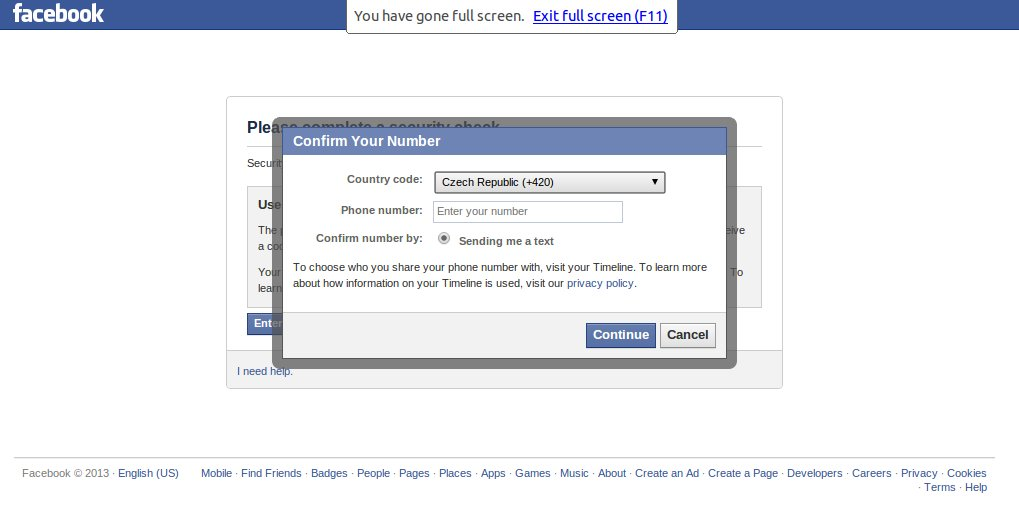
\includegraphics[width=5in]{figures/fb-telephone-number2.jpg}
\caption{Zadávání telefonního čísla na facebooku}
\label{fig:fbTelephoneNubmer}
\end{center}
\end{figure}

Nejdříve bylo potřeba založit e-mailové adresy, sloužící k vytvoření falešných účtů na facebooku. 
Všechny e-mailové adresy byly založeny na české doméně a měly koncovku \verb|.cz|, protože jsem chtěl provést experiment na uživatelích facebooku z České republiky, aby bylo vše věrohodnější.
Pro vytváření e-mailových adres jsem použil především bezplatnou e-mailovou službu od portálu seznam.cz (jedná se v první řadě o internetový vyhledavač, e-mailové schránky jsou provozovány jako jedna z doplňkových služeb). 
Na tomto portálu lze vytvářet e-mailové adresy s koncovkou \verb|@seznam.cz| a \verb|@email.cz|.

Pro každý falešný účet na facebooku jsem nejdříve připravil náhodné jméno a příjmení. 
Hlavním požadavkem na jméno bylo, aby bylo co nejvíce náhodné, ale zároveň i uvěřitelné. 
Nechtěl jsem proto vytvářet nová jména, ale raději využít již existující.
Ve velkém množství případů se jednalo o spojení různých křestních jmen a příjmení získaných ze stažených facebookových profilů.
U některých jmen byl změněn i rod příjmení.
Nadále jsem pro vytváření jmen použil službu \verb|www.zlatestranky.cz|\footnote{Jedná se o internetový seznam telefonních čísel fyzických a právnických osob v České republice} (v současné době stránky obsahují pouze seznam právnických osob a změnila se grafika celých stránek, ale v době kdy jsem účty zakládal byl na stránkách i seznam fyzických osob).

Struktura e-mailových adres byla následující: \verb|jmenoprijmeni@domena|. Přednost měla doména \verb|seznam.cz|, pokud byla e-mailová adresa s tímto jménem již zabraná, použil jsem doména \verb|email.cz| a pokud nebyla k dispozici ani tato e-mailová schránka, tak se za jméno vložila číslice (například: jannovak5@seznam.cz) anebo byla použita modifikace křestního jména (domácký výraz, zdrobnělina a podobně).

Při vytváření e-mailových adres jsem na žádná omezení nenarazil. Webových stránek nabízejících bezplatně e-mailové adresy je velké množství a to i pokud potřebujeme e-mailovou adresu pouze z české domény. Po úspěšné registraci na facebook bylo vždy potřeba aktivovat pomocí e-mailu. Facebook ihned po registraci zašle na e-mail zadávaný při registraci zprávu s odkazem. Aktivace účtu probíhá otevřením ověřovacího odkazu z e-mailu.

Facebook poté na zadaný e-mail posílá upozornění na různé aktivity, které se na facebooku dějí (například žádost o přátelství, zaslání zprávy apod.). Typy zasílaných zpráv z facebooku lze nastavit v uživatelském nastavení. Pro experiment byly e-mailové adresy důležité pouze pro povolení facebookového účtu.

\subsection{Internetové služby poskytující dočasné e-mailové schránky}
Před začátkem experimentu jsem uvažoval nad použitím některé ze služeb pro dočasné e-mailové adresy. Jedná se o služby, které vám při návštěvě vygenerují náhodnou e-mailovou adresu (například:\newline \verb|e1461664@rmqkr.net|). Takovéto e-mailové adresy fungují jen po omezeně dlouhou dobu a všechy e-mailové zprávy, které jsou odeslány na tuto adresu se zobrazí přímo na navštívené stránce (pouze pro návštěvníka, pro kterého byla daná e-mailová adresa vygenerována). Příklady dočasných e-mailových služeb: \verb|http://10minutemail.com/|, \verb|http://mailinator.com/|,\newline \verb|https://meltmail.com/| a další.

Zjistil jsem ale, že facebook registrace z takovýchto dočasných e-mailových adres blokuje a po registraci je potřeba zadat telefonní číslo, na které příjde ověřovací kód, stejně jako při registraci více účtů z jedné IP adresy. Také se mi nepodařilo najít službu s dočasnými e-mailovými adresami, které by obsahovly doménu s koncovkou \verb|.cz|. Použil jsem proto služby českých e-mailových serverů. Hlavní výhodou je to, že k e-mailovým schránkám budu mít přístup i později a nebude problém pokud by bylo potřeba dohledat některé informace posílané e-mailem (například zapomenuté heslo nebo důvod zablokování facebookového účtu).

\section{Problémy se zakládáním facebookových účtů}

Zakládal jsem tedy profily na facebooku již dopředu, abych mohl experiment spustit najednou ve stejný čas. 
Bohužel se mi ale stalo to, že dříve založené účty na facebooku byly neaktivní a když jsem se k nim přihlásil po nějáké době, tak facebook požadoval zadání telefonního čísla, pro ověření totožnosti uživatele (stejně jako pokud se pokoušíme zaregistrovat více účtů denně z jedné IP adresy). Problém byl v tom, že facebook bere účty jako věrohodné až   pokud má několik přátel a vyvíjí aktivitu na facebooku.

Stalo se tedy to, že jsem zakládal účty, aktivoval jsem je pomocí e-mailové adresy, ale už na účtech nebylá žádná další aktivita. Když jsem se poté v den spouštění experimentu k účtům vrátil, tak se mi objevilo textové pole s prosbou o ověření účtu zadáním telefonního čísla. Musel jsem tedy spustit experiment jen s funkčními účty s tím, že jsem po spuštění experimentu zakládal další nové účty.

Teoreticky by bylo možné celý proces zakládání účtů plně zautomatizovat. E-mailové adresy pro registrované účty by šlo jenoduše zařídit na vlastní doméně nastavením doménového koše. To znamená, že veškeré e-maily, které byly odeslané na adresu naší domény budou doručeny na jednu konkrétní e-mailovou adresu. Získáme tak teoreticky neomezené množství e-mailů k registraci na facebook.

Dále by se musel vyřešit problém s registrací z jedné IP adresy denně. Toto omezení by šlo obejít použitím několika spolehlivých proxy serverů\footnote{Proxy server - server, prostřednictvím kterého se lze připojit k internetu, výhodou je že není vidět naše IP adresa, ale IP adresa proxy serveru, seznam proxy serverů lze nalézt na internetu, například - http://www.hidemyass.com/proxy-list/}, přes které by byly falešné účty registrovány. Rychlost registrovaných účtů na facebooku denně by se odvíjela od počtu využívaných proxy serverů. 

Pravděpodobně by se muselo vyřešit i opisování kontrolního CAPTCHA kódu, pokud facebook detekuje podezřelou robotickou činnost. Na internetu ale fungují služby, které umí za poplatek řešit opisování CAPTCHA obrázků\footnote{http://decaptchablog.com/decaptcher-services}. Vše funguje automaticky pomocí OCR (Optical character recognition - optické rozpoznávání znaků) anebo lidským opisováním textů. Výhodou takovýchto služeb je, že si lze vše pronajmout a nemusíme se starat o nic jiného.

Pravděpodobně by bylo potřeba řešit i jiné problémy spojené s automatickým zakládáním facebookových profilů, které by se objevily při hlubším bádání nad problémem. Každopádně se ale určitě jedná o velmi zajímavé téma, které by šlo zpracovat více do hloubky. Protože by rozsah takovéhoto rozpracování pravděpodobně vydal na samostatnou diplomovou práci. Já jsem pro svůj experiment potřeboval pouze omezený počet facebookových účtů, takže jsem všechny účty zakládal ručně.

[todo]
- etika = ovladani v pohode?
- seznam uzivatelu = jen data

\section{Strategie přidávání přátel k falešným účtům}

Při vymýšlení celého experimentu bylo hlavním cílem simulovat reálné chování uživatelů na facebooku. Chtěl jsem také vyzkoušet různé strategie přidávání přátel. Na začátku experimentu jsem tedy rozdělil všechny účty do pěti kategoríí podle vyplněnosti profilu. Každá kateogie měla známku od 1 do 5, přičemž známka 1 znamená, že profil je nevyplněný a známka 5 znamená, že profil je velmi vyplněný. Hlavní motivací pro takovéto rozdělení je, že více vyplněné facebookové profily by měly být pro ostatní návštěvníky věrohodnější.

Faktory ovlivňující vyplněnost profilu:

- profilový obrázek a  

- foto
- 5 skupin
- 5 levelu
- ucty se navzajem neznaji




%\begin{conclusion}
%\end{conclusion}
\chapter{Z{\' a}v{\v e}r}


\section{Vyhodnocení}
- Grafy
- Vyhodnocení


\section{Možnosti pokračování experimentu}

Pro naši aplikaci nebylo potřeba uchovávat texty komentářů u statusů, takže se tento problém nemusel řešit. Ukládá se pouze počet komentářů, který lze získat zpracováním zobrazeného textu. Ukládání textu komentářů by mohlo být užitečné, pokud by bylo možné zjistit citové zabarvení komentářů (negativní/pozitivní/neutrální). Pro takovéto analýzy jsou ale potřeba pokročilé algoritmy pro práci s textem a pro kvalitní rozpoznání by bylo potřeba delší úseky textu. Takovéto analýzy se využívají pro sledování nálady ve společnosti (například při volbách apod.) anebo pro sledování spokojenosti s určitým produktem nebo brandem (značkou) na sociálních sítích. 

Hlavní cíl experimentu ale byl odlišný a počet facebookových účtů, které byly do experimentu zahrnuty nebyl dostatečně velký (hlavně počet facebookových přátel účtů), aby měly výsledky vypovídající hodnotu. Každopádně by se při větším množství účtů zahrnutých do experimentu mohlo podařit získat vypovídající masu lidí, kde by mohly být výsledky zajímavé. Zatím jsou takováto data získávána pouze z veřejně dostupných zdrojů anebo ze stránek na facebooku a takováto data mohou být zkreslená (omezením vzorku jen na určitou skupinu uživatelů). Jedná se o jeden ze směrů, kterým by se dal experiment dále rozšířit a pokračovat v něm v budoucnu.

Kromě získávání nálady ve společnosti by bylo možné i ovlivňovat ostatní profily. Vkládáním pozitivních statusů o určitém příspěvku by mohlo sloužit jako zajímavá reklama. Lidé jsou odmítaví ke klasickým formám reklamy (letáky, televizní reklamy, apod.), ale pokud by se jednalo o pozitivně laděné sdělení, které by nevypadalo na první pohled jako reklama, mohlo by se jednat o zajímavou možnost ovlivnit mínění facebookových uživatelů. Teoreticky by nemuselo být sdělení pozitivní, někdy by mohla stačilt zmínka na facebooku a uživatelé by se díky sociální aktivitě (sdílení, dávání like a komentování) postarali o šíření mezi další uživatele internetu. Reklama by mohla být i negativní. V dnešní době už existují služby pro placené blogové články na míru (Například \verb|placla.cz|). Podobně by to mohlo fungovat i u facebooku.

Facebook na podzim roku 2012 zavedl možnost placení za zviditelnění statusů. Na facebooku se nyní nezobrazují všechy statusy od vašich přátel, ale jen vybrané statusy, které facebook považuje pro vás za nejhodnotnější a nejkvalitnější. Vše jde nastavit a ovlivnit skupinami do kterých si přátele zařadíte (algoritmy pro zobrazování příspěvků nejsou veřejné). Nikdy ale nemáte jistotu, že váš příspěvek uvidí všichni (nebo určití) přátelé. Za poplatek \$6.99 (přibližně 140 Kč - duben 2013) pak uživaté facebooku mohou promovat své příspěvky, aby se zobrazily většímu počtu kamarádů. Takto lze promovat příspěvky i u facebookových stránek, kde tato funkce dává větší smysl.


[TODO] zdroje/citace??? :)
\bibliographystyle{csn690}
\bibliography{mybibliographyfile}

\appendix

\chapter{Slovník použitých pojmů a zkratek}
%\printglossaries
\begin{description}
	\item[HTML] - Hypertext markup language - zdrojový formát vzhledu webových stránek, který je zpracováván internetovým prohlížečem
		\newline(http://en.wikipedia.org/wiki/HTML).
	\item[Like skupiny na facebooku] - Like = Líbí se mi - způsob připojení se ke skupně (Group) nebo stránce (Page) na facebooku
	\item[Like statusu] - Like = Líbí se mi - způsob vyjádření, že se uživatelovi líbí status na facebooku, bez nutnosti status komentovat. Jedná se o modré tlačítko, na kterém je znázorněn palec nahoru.
	\item[Postování statusu] - Vkládání příspěvku na svou zeď na  facebooku.
	\item[Přidat se do vztahu na facebooku] - 
	\item[Přítel na facebooku] - Jedá se o virtuální kamarádství mezi dvěma lidmi, které funguje tak, že oba zúčastnění musí přátelství potvrdit. Prakticky vše probíhá tak, že můžeme komukoliv na facebooku zaslat pozvánku k přátelství, dotyčný pak může pozvánku přijmout anebo odmítnout.  
	\item[Profil na facebooku]
	\item[(internetový) prohlížeč = browser] - Program pro zpracování a zobrazování internetových stránek. Zpracovává takzvaný HTML kód webové stránky.
	\item[REST] - Representational state transfer - Architektura rozhraní pro komunikaci s webovými službami (Web services), postavený nad HTTP protkolem
\newline(https://en.wikipedia.org/wiki/Representational\_state\_transfer).
	\item[Status] - Příspěvek na svou facebookovou zeď od uživatelů (Facebook nabádá k odpovědi na otázku: „What is on your mind?“ = „Co se vám honí hlavou?“).
	\item[Stránka na facebooku]
	\item[Šťouchnout na facebooku (Poke)] -
	\item[Zeď na facebooku] - V terminologii facebooku se zeď používá k označení seznamu příspěvků svých a svých kamarádů.
\end{description}

\chapter{Obsah přiloženého CD}

\begin{figure}
	\dirtree{%
		.1 readme.txt\DTcomment{stručný popis obsahu CD}.
		.1 exe\DTcomment{adresář se spustitelnou formou implementace}.
		.1 src.
		.2 impl\DTcomment{zdrojové kódy implementace}.
		.2 thesis\DTcomment{zdrojová forma práce ve formátu \LaTeX{}}.
		.1 text\DTcomment{text práce}.
		.2 thesis.pdf\DTcomment{text práce ve formátu PDF}.
		.2 thesis.ps\DTcomment{text práce ve formátu PS}.
	}
\end{figure}

\end{document}
